\documentclass{beamer}
\usepackage{ctex}
\mode<presentation>
{
  \usetheme{Madrid}      % or try Darmstadt, Madrid, Warsaw, ...
  \usecolortheme{beaver} % or try albatross, beaver, crane, ...
  \usefonttheme{default}  % or try serif, structurebold, ...
  \setbeamertemplate{navigation symbols}{}
  \setbeamertemplate{caption}[numbered]
} 

\usepackage[utf8]{inputenc}
\usepackage[T1]{fontenc}

\title[Social evolution, mask wearing, \& epidemics]{Social evolution, mask wearing, and epidemics}
\author{修格致}
\institute{IRSGIS, Peking Univ.}
\date{\today}

\begin{document}

\begin{frame}
  \titlepage
\end{frame}

\begin{frame}{Outline}
 \tableofcontents
\end{frame}

\section{Introduction}

\begin{frame}{Introduction}
\vspace{0.5cm}
    What is the impact of \textit{adaptive social relations} on pandemics

\begin{itemize}
  \item `Peer pressure' on wearing protections?
  \item How you will react to those silly people?
\end{itemize}
\vspace{1cm}

Concerns

\begin{itemize}
    \item Social structures
    \item Epidemic spread with protections
    \item Bifurcations
    \item \textbf{Micro-structure behind epidemic threshold?}
\end{itemize}

\end{frame}

\section{Logics}

\subsection{Graph fission}

\begin{frame}{Graph fission}

\begin{itemize}
    \item 演化图:节点恒定,而连边方式随时间变化的图结构。
    \item Multiplex network:节点给定,而连接属性多于一个。
\end{itemize}
\begin{figure}
\centering
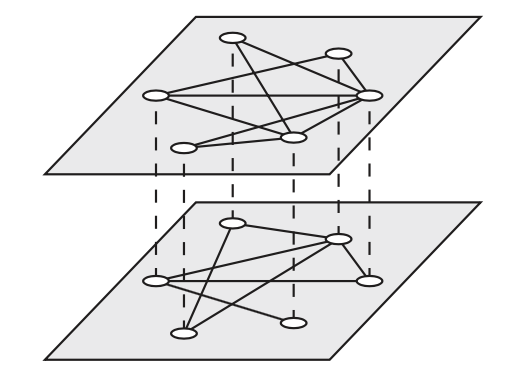
\includegraphics[width = 0.5\linewidth]{figs/截屏2020-07-10 下午7.11.46.png}    
\end{figure}

\end{frame}

\begin{frame}{Graph fission}

\begin{itemize}
    \item 演化图:节点恒定,而连边方式随时间变化的图结构。
    \item Multiplex network:节点给定,而连接属性多于一个。
    \item \textbf{图裂变:图从连通图变为非连通图的过程。}
    \begin{itemize}
        \item 常见类型:渗流、voter模型、Ising模型、自旋模型等
    \end{itemize}
\end{itemize}
\end{frame}

\begin{frame}{Graph fission}

\begin{itemize}
    \item 为什么要研究图裂变?
    \begin{itemize}
        \item 概括性:网络拓扑的演化使得网络的局部性质与全局性质不统一,子采样的结果不再成立
        \item 适合性:真实世界中,人们的观点、行为、意识割裂严重,需要合适的数学模型来反映
        \item 时态性:由于网络演化的速度不同,不同时段的网络性质的连续变化往往不可以用收敛后的结果来覆盖,而需要合适的收敛速度分析指标。
    \end{itemize}
\end{itemize}
\end{frame}

\begin{frame}{Graph fission}
    \begin{figure}
        \centering
        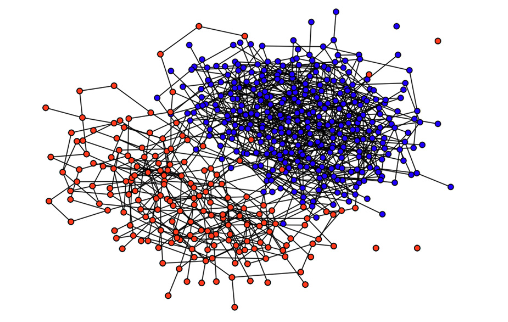
\includegraphics[width = 0.8\linewidth]{figs/截屏2020-07-10 下午7.23.09.png}
        \caption{\textbf{Right before Graph fission.} \textit{Graph fission in an evolving voter model, PNAS 2012, Durrett et. al.}}
    \end{figure}
\end{frame}
%%%% 
\subsection{Related}
\begin{frame}{Graph fission \& Voter model}
一个基本的例子:
\begin{itemize}
    \item a social network in which individuals have one of two opinions (called 0 and 1) 
    \item their opinions and the network connections coevolve
    \item 随机在网络中选边,如果边的两侧意见不同:
    \begin{itemize}
        \item 概率$1-\alpha$: 一个模仿另一个;
        \item 概率$\alpha$: 两个人不联系,其中一个人随便找一个别人交往。
        \begin{itemize}
            \item 子模型1: 选相同意见的
            \item 子模型2: 随机选人交往
        \end{itemize}
    \end{itemize}
    \item 最终图\textit{可能}会分化为两个不相连接的子图。
    \end{itemize}    
\end{frame}
\begin{frame}{Graph fission \& Epidemics}
另一个例子
\begin{itemize}
    \item The nodes represent individuals, which are either susceptible (S) or infected (I). 
    \item In every time step and for every link connecting an infected with a susceptible (SI link), the susceptible becomes infected with the fixed probability p. The Infected recovers from the disease with probability r, becoming susceptible again.
    \item Allowing susceptible individuals to protect themselves by rewiring their links. With probability w for every SI link, the susceptible breaks the link to the infected and forms a new link to another randomly selected susceptible. 
\end{itemize}
    
\end{frame}
%%%% 
\section{社会并不如此简单}
\subsection{非对称的社会影响力}
\begin{frame}{不公平条件下的社会会面临什么问题?}
上述模型中,演化总是\textbf{对称的},即相互同化的概率是相同的。
\vspace{1cm}
    \begin{itemize}
    \item 这显然过于理想!
    \vspace{1cm}
    \pause
    \item 如果两种意见相互影响的程度不同,结果会怎样?
    \item 如果两种意见不止控制了一个传播过程,也对另一个传播过程产生影响,结果会怎么样?
\end{itemize}
\end{frame}

\begin{frame}{我们的模型:口罩驱动社交关系变化}
\begin{block}{Key:}
    \textit{戴口罩}对于人的社交关系和疾病传播都有影响。戴口罩可以降低被传染的风险;也可以让你识别出真正与自己有共同认知的人。
\end{block}
\pause
\vspace{1cm}
\begin{itemize}
    \item 两个效应:
    \begin{itemize}
        \item 分隔效应:戴口罩跟戴口罩玩,不戴口罩跟不戴的玩。
        \item 同化效应:不戴口罩的比戴口罩`凶',在线下沟通的时候,不戴口罩的人会越变越多。
    \end{itemize}
\end{itemize}
\end{frame}

\begin{frame}{我们的模型:口罩驱动社交关系变化}
    \begin{itemize}
        \item We consider a network with $N$ nodes representing individuals, and $K$ links representing the social contacts. 
        \item Each of the individuals has two attributes. They are either susceptible (\textit{S}) or infected (\textit{I}), and either pro (\textit{P}) or con (\textit{C}) for wearing facial masks. 
        \item On a link connecting an \textit{I} node with an \textit{S} node, the \textit{S} node becomes infected with rate $\mu$ if the S node is not wearing a mask, and $\gamma \mu$ if the S node wears a mask for $\gamma < 1$. The \textit{I} node recovers with rate $r$. 
        \item The interactions also serve as the media of attitudes towards masks. If a link is discordant of the opinions of wearing masks, they become both $P$ nodes with rate $\beta_1$, and that of both $C$ nodes with rate $\beta_2>\beta_1$. They stop seeing each other and one of them finds a new random interaction with rate $1-\beta_1-\beta_2$.
        \begin{itemize}
            \item The random picks studied here lie in two ways, (i) rewire-to-same, i.e., picking a node that shares the same opinion; and (ii) rewire-to-random, i.e., picking a random node over the graph. 
        \end{itemize}
    \end{itemize}
\end{frame}


\begin{frame}{Results: Network Topology}
    \begin{figure}
        \centering
        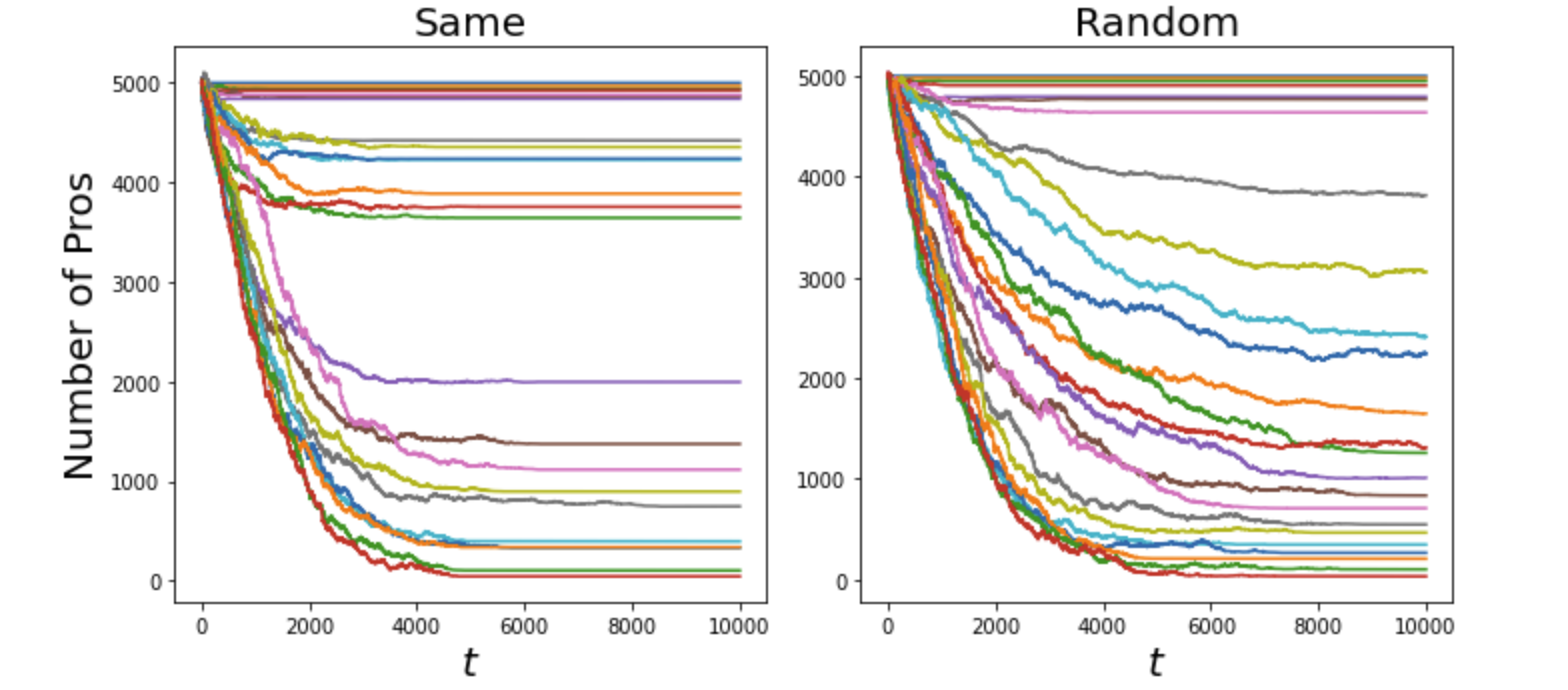
\includegraphics[width = 0.8\linewidth]{figs/截屏2020-07-10 下午7.57.32.png}
        \caption{Supportive for Masks as a function of time.}
    \end{figure}
    进一步,戴口罩的人群的连通度也比较低。
\end{frame}
\subsection{社会是否会疏离?}
\begin{frame}{社会是否会疏离?}
真的会戴口罩与戴口罩玩,不戴口罩跟不戴口罩的玩吗?
    \begin{itemize}
        \item 收敛速度:拟合+理论:达到社会共识(不戴口罩)$T \simeq N^{3/2}$
        \item 是否可以收敛:To illustrate the reason behind this, we recall the voter model on the d-dimensional lattice $\mathbb{Z}^d$ (See Ref [15] for details.): For $d \le 2$, the voter model convergent complete consensus, i.e., if $x\ne y$, then $P[(\xi_t)\ne \xi_t(y)]\to 0$.
    \end{itemize}
\end{frame}

\subsection{疏离的后果?}
\begin{frame}{社会分隔,Then what?}
两个群体的Epidemic threshold不一样:
\begin{itemize}
    \item 正常图的临界传播概率设为$p^*$.
    \item 临界条件:$R_0 = p\langle k \rangle / r = 1$
    \item 有重连:$k(t) = \langle k \rangle\exp(-wt)$, 节点患病的期望时间:$1/r$
    \item 临界传染率:\begin{align*}
        p^* = \frac{w}{\langle k \rangle[1-\exp(-w/r)]}
    \end{align*}
\end{itemize}
\begin{center}
    戴口罩的人群 $p$更低,所以更不容易达到临界传染率。
\end{center}
\end{frame}

\begin{frame}{Degree distribution}
    \begin{figure}
        \centering
        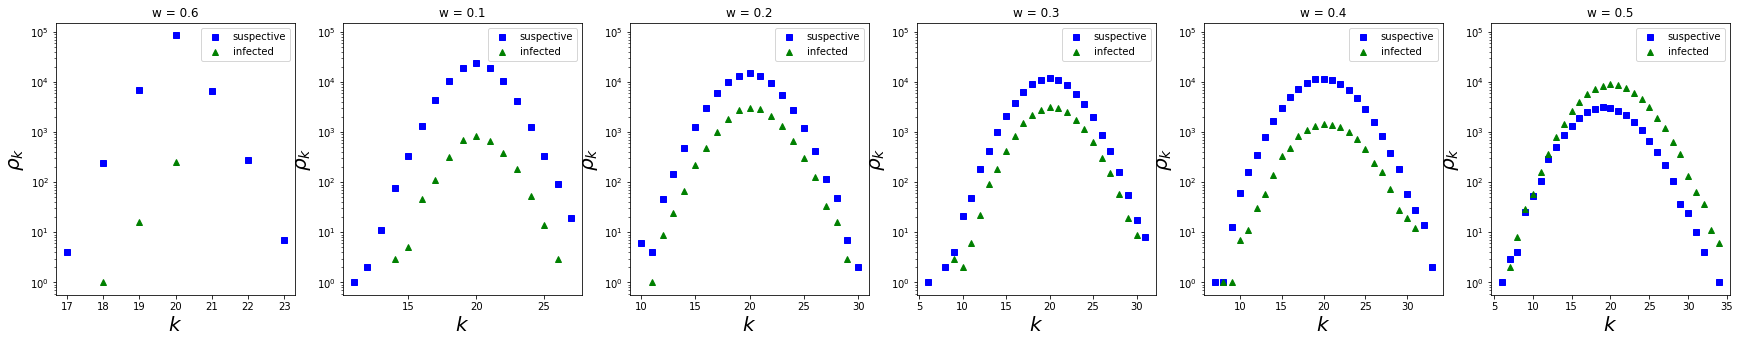
\includegraphics[width = 0.5\linewidth]{figs/degreedistsi.png}
    \end{figure}
\end{frame}

\begin{frame}{Degree distribution standardized}
    \begin{figure}
        \centering
        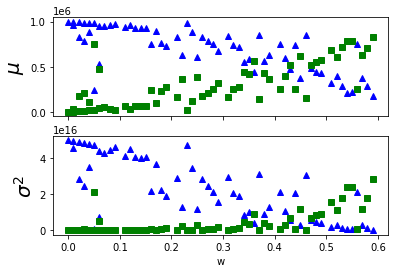
\includegraphics[width = 0.5\linewidth]{figs/degreediststandardized (1).png}
    \end{figure}
\end{frame}

\begin{frame}{模型的极限}
戴口罩就万事大吉啊了吗?
\begin{itemize}
    \item 不是的,有可能会出现疾病分岔的局面。
\end{itemize}
\begin{figure}
    \centering
    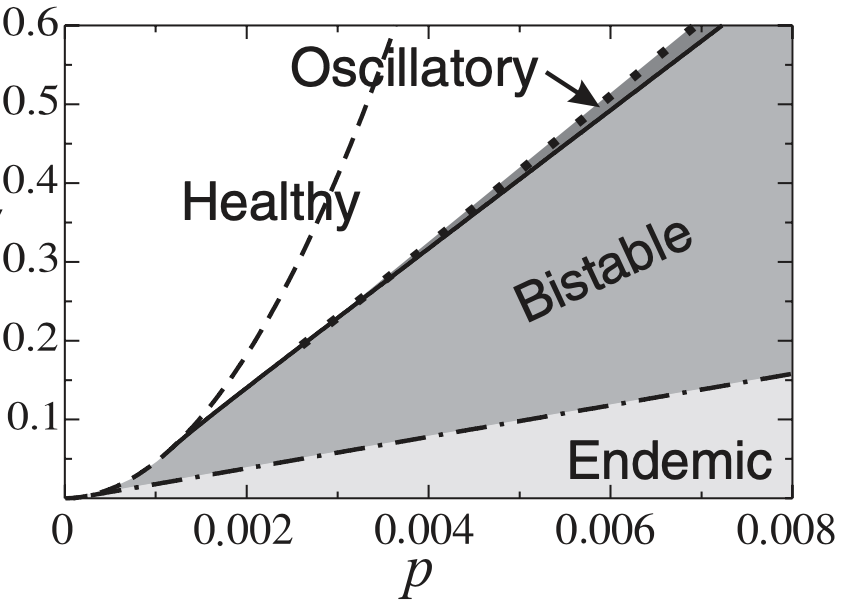
\includegraphics[width = 0.6\linewidth]{figs/截屏2020-07-10 下午8.18.02.png}
\end{figure}
\end{frame}

\section{总结}

\begin{frame}{总结:不平等的意义?}

\begin{itemize}
    \item 群体内部的一些不平等实际上有助于确保每个人都有可能不生病
    \item 即使统计数据失效,小群体内的共识依然是有意义的
\end{itemize}
\begin{center}
    什么情况下,不平等有害,什么情况下,不平等也会变得有益?
    
    \vspace{1cm}

    \textbf{清者自清}
\end{center}
    
\end{frame}
\end{document}
